% !TEX root = ../../main.tex
\section{Artifical data generation}\label{sec:artificial_data_generation}
\TODO{Use data from \cite{camci2010change,takeuchi2006unifying}}
In this section we present three data sets as used by \cite{camci2010change,takeuchi2006unifying} to provide for a objetive performance comparison.

Model:
\begin{equation}
  x_t = a_1 x_{t-1} + a_2 x_{t-2} + \epsilon_t,
\end{equation}
where $\epsilon_t$ is a Gaussian distribution, modeling the noise.
The length of $x_t$ is $10000$ and change points are generated at each $y \times 10000^\text{th}$ data point, with $y = (1, 2, 3, \dots 9)$.

First Takeuchi, reduced jumping mean:
$\epsilon_t$ is Gaussian with mean $0$ and variance $\sigma^2 = 1$, $a_1 = 0.6$ and $a_2 = -0.5$.


First Camci, fixed jumping mean.
$\Delta y = 5$
See Figure~\ref{fig:camci_mean_fixed}.


\begin{figure}
\centering
  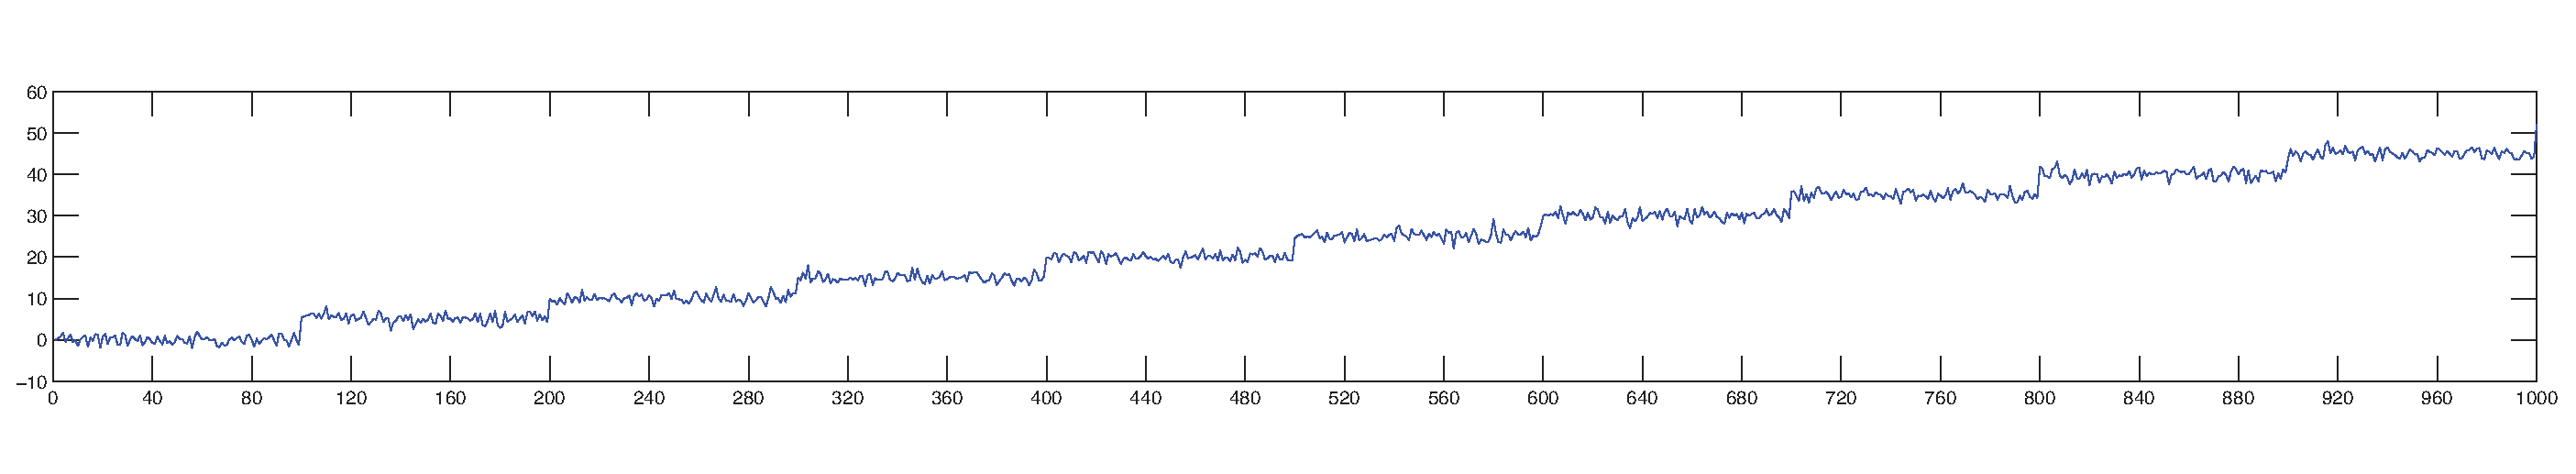
\includegraphics[width=1\textwidth]{./Figures/notes/jumping_mean_camci.eps}
  \caption[Jumping mean camci]{Jumping mean camci}
  \label{fig:camci_mean_fixed}
\end{figure}

\begin{figure}
\centering
  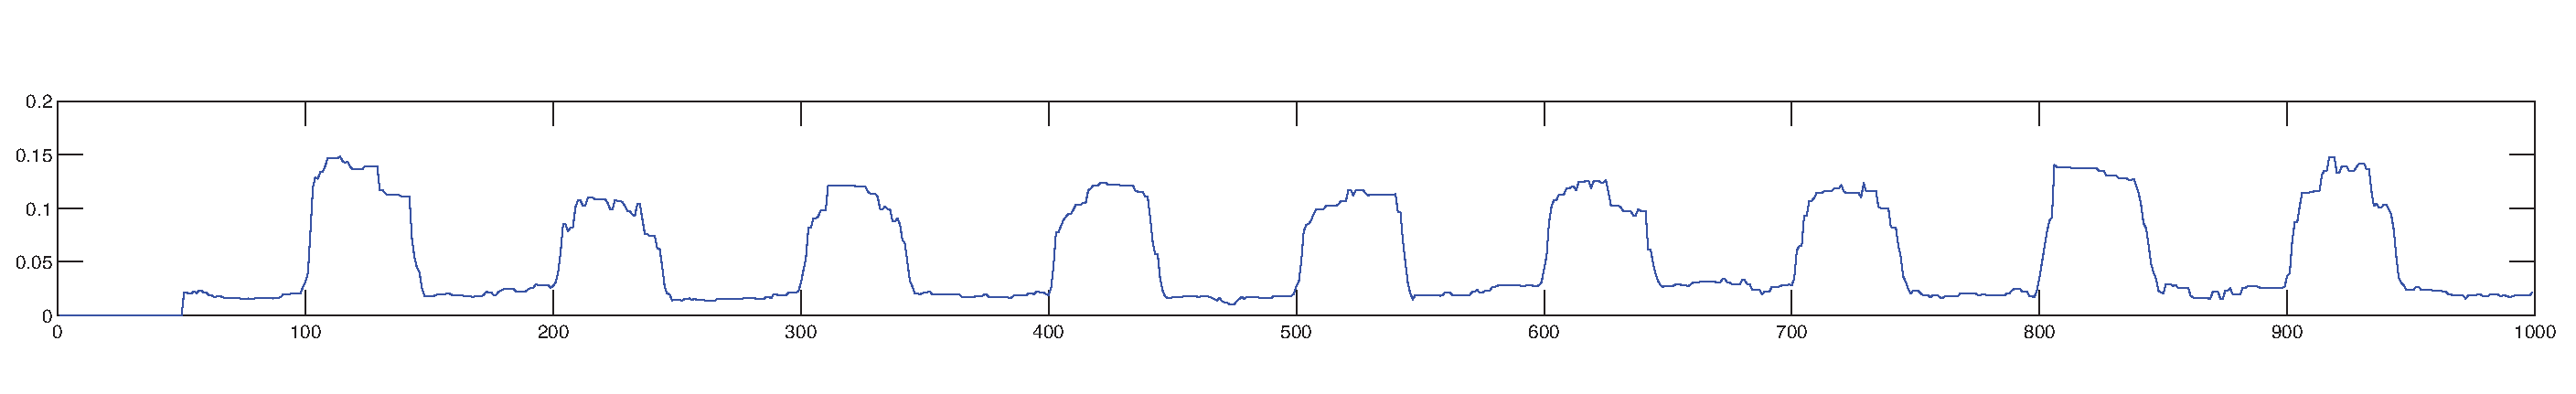
\includegraphics[width=1\textwidth]{./Figures/notes/jumping_mean_camci_thresholds.eps}
  \caption[Jumping mean camci thresholds]{Jumping mean camci, thresholds}
\end{figure}

\begin{figure}
\centering
  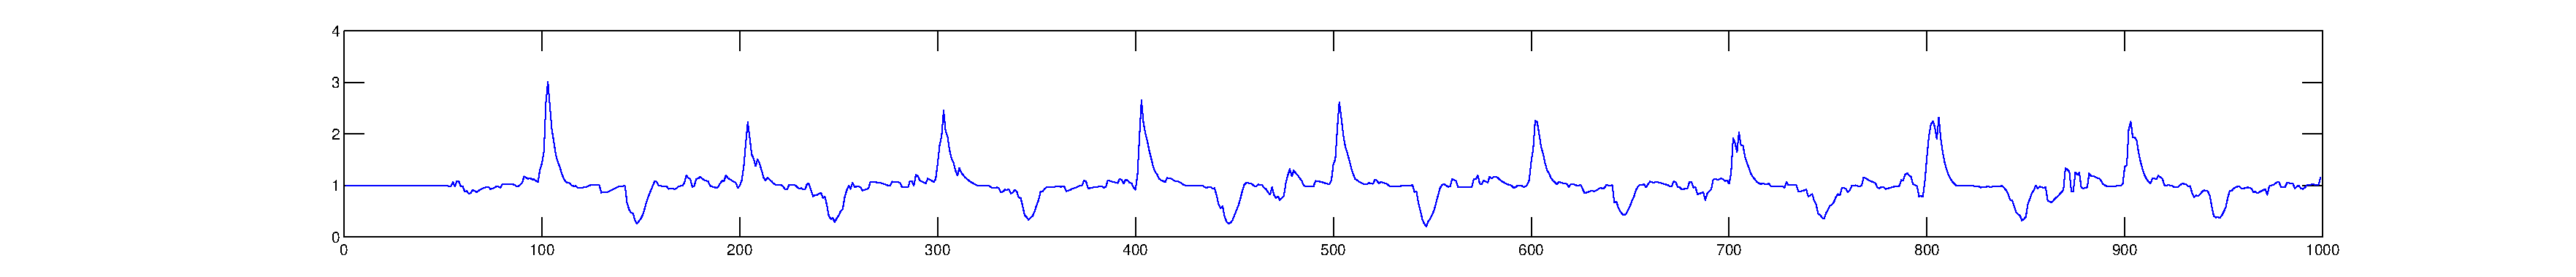
\includegraphics[width=1\textwidth]{./Figures/notes/jumping_mean_camci_ratios_10.eps}
  \caption[Jumping mean camci ratios]{Jumping mean camci ratios, last 10}
  \label{fig:jumping_mean_ratios}
\end{figure}

\begin{figure}
\centering
  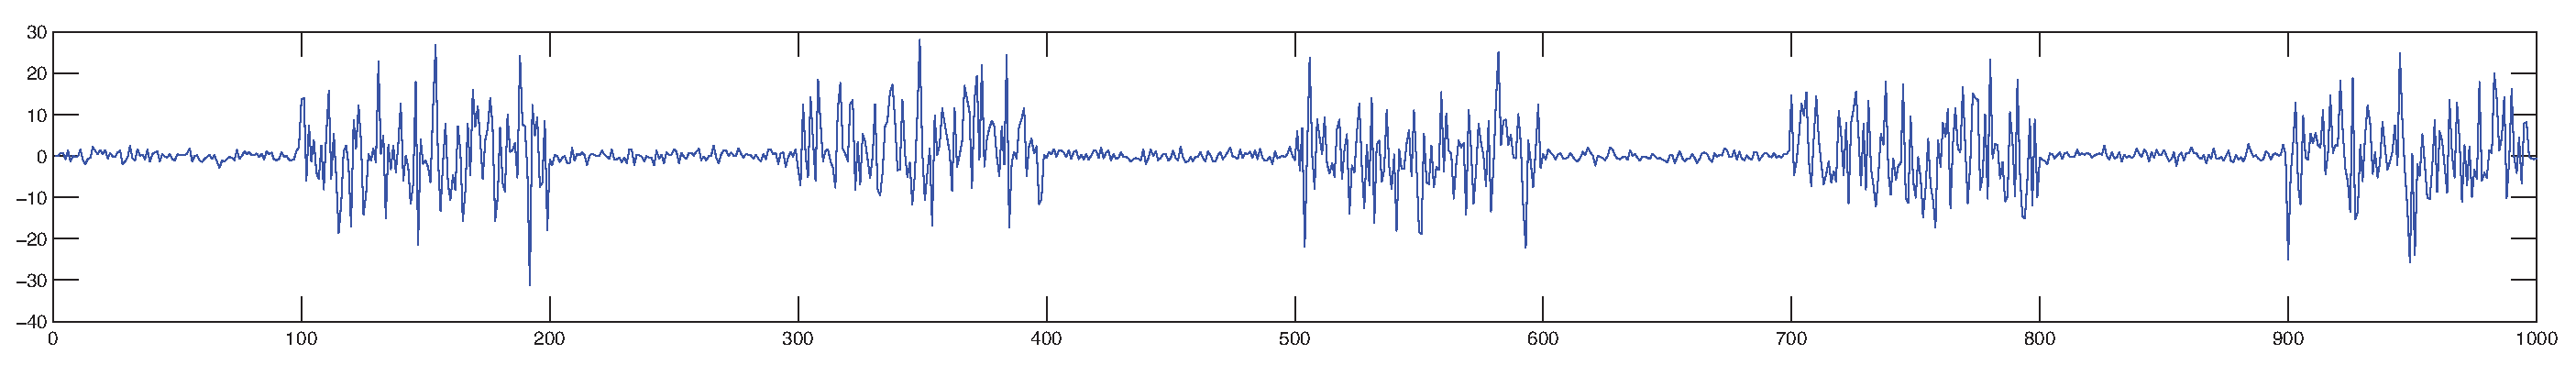
\includegraphics[width=1\textwidth]{./Figures/notes/jumping_variance.eps}
  \caption[Jumping variance]{Jumping variance}
\end{figure}

\begin{figure}
\centering
  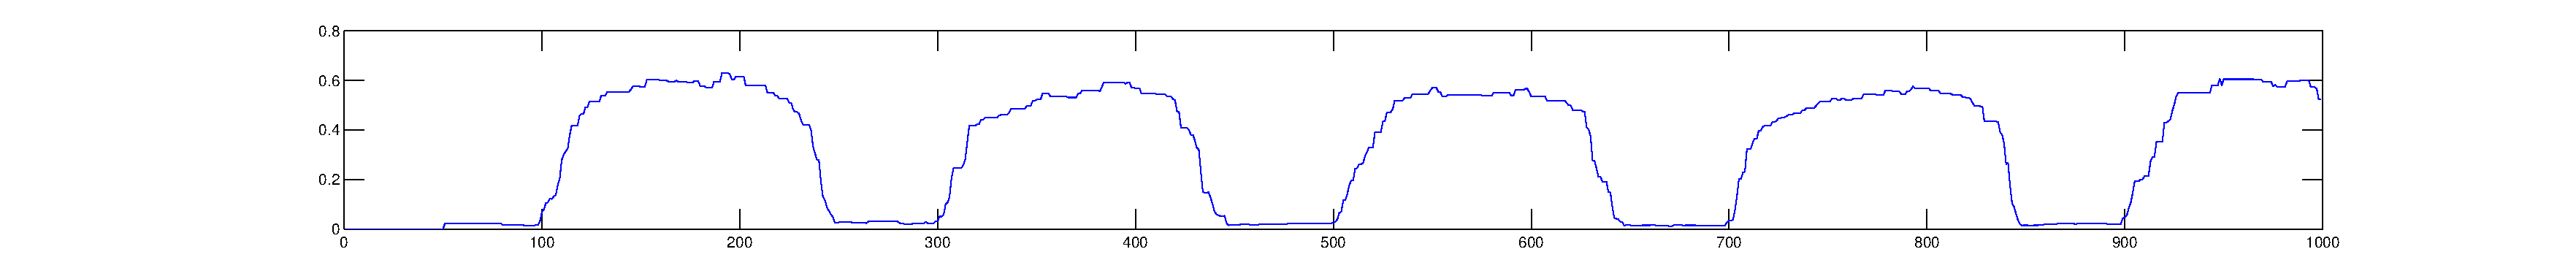
\includegraphics[width=1\textwidth]{./Figures/notes/jumping_variance_thresholds.eps}
  \caption[Jumping variance thresholds]{Jumping variance, thresholds}
\end{figure}

\begin{figure}
\centering
  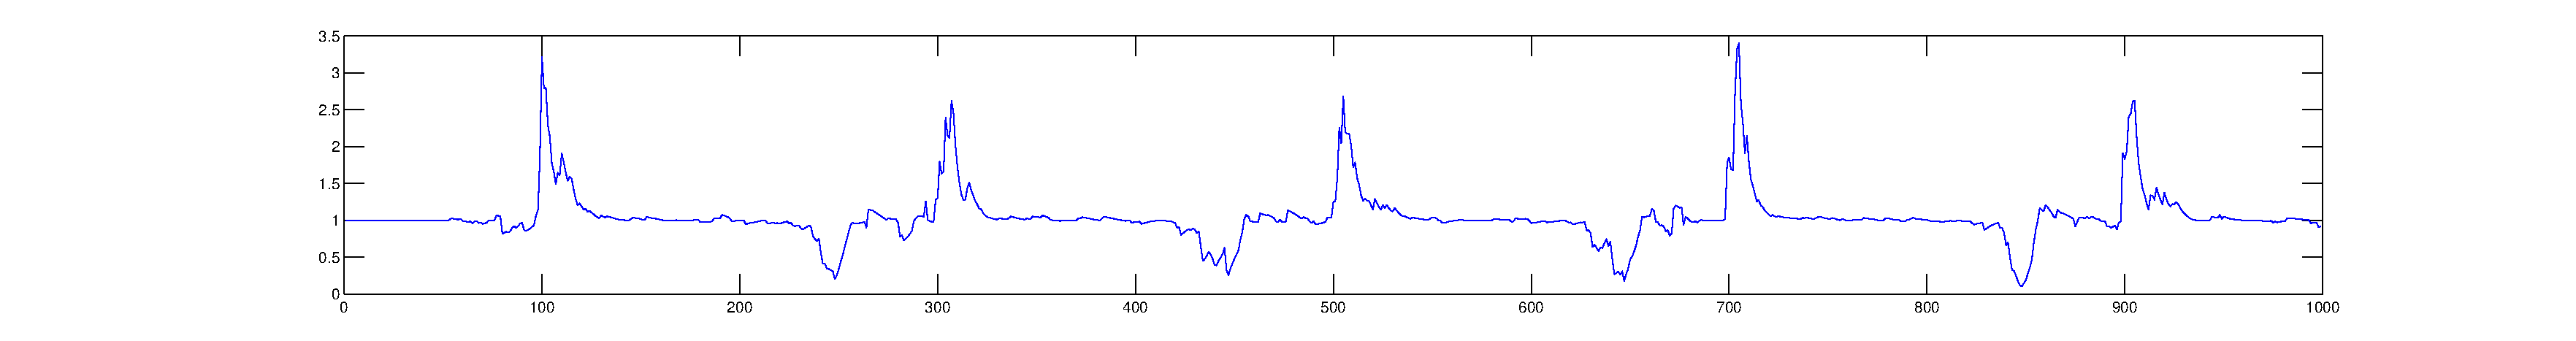
\includegraphics[width=1\textwidth]{./Figures/notes/jumping_variance_ratios_10.eps}
  \caption[Jumping variance ratios]{Jumping variance ratios, last 10}
\end{figure}